\documentclass{article}

\usepackage{mathpartir}
\usepackage{amssymb}
\usepackage{graphicx}

\newcommand{\ternary}[3]{{#1}\ \mathjs{?}\ {#2}\ \mathjs{:}\ {#3}}
\newcommand{\funcall}[2]{{#1}\mathjs{(}{#2}\mathjs{)}}
\newcommand{\paren}[1]{\mathjs{(}{#1}\mathjs{)}}
\newcommand{\dom}{\mathit{dom}}
\newcommand{\funtype}{\mathit{fun}\mbox{-}\mathit{type}}
\newcommand{\vartype}{\mathit{var}\mbox{-}\mathit{type}}
\newcommand{\rettype}{\mathit{return}\mbox{-}\mathit{type}}
\newcommand{\funty}[2]{({#1}) \rightarrow {#2}}
\newcommand{\seq}[1]{\overline{{#1}}}
\newcommand{\mathjs}[1]{\mbox{\texttt{{#1}}}}
\newcommand{\mathjssm}[1]{\mbox{\texttt{\scriptsize {#1}}}}
\newcommand{\return}[1]{\mathjs{return }{#1}\mathjs{;}}
\newcommand{\fun}[3]{\mathjs{function }{#1}\mathjs{(}{#2}\mathjs{) \char123{} }{#3}\mathjs{ \char125{}}}
\newcommand{\afun}[2]{\mathjs{function}\mathjs{(}{#1}\mathjs{) \char123{} }{#2}\mathjs{ \char125{}}}
\newcommand{\var}[1]{\mathjs{var }{#1}\mathjs{;}}
\newcommand{\rel}[1]{\scriptsize [\textsc{#1}]}
\newcommand\defeq{\stackrel{\mbox{\tiny def}}{=}}
\newcommand{\while}[2]{\mathjs{while (}{#1}\mathjs{) }{#2}}
\newcommand{\dowhile}[2]{\mathjs{do }{#1}\mathjs{ while (}{#2}\mathjs{);}}
\newcommand{\for}[4]{\mathjs{for (}{#1}\mathjs{; }{#2}\mathjs{; }{#3}\mathjs{) }{#4}}
\newcommand{\switch}[2]{\mathjs{switch (}{#1}\mathjs{) \char123{} }{#2}\mathjs{ \char125{}}}
\newcommand{\switchdef}[3]{\mathjs{switch (}{#1}\mathjs{) \char123{} }{#2}\mathjs{ default:}\,{#3}\mathjs{ \char125{}}}
\newcommand{\brk}{\mathjs{break;}}
\newcommand{\brkl}[1]{\mathjs{break }{#1}\mathjs{;}}
\newcommand{\cont}{\mathjs{continue;}}
\newcommand{\contl}[1]{\mathjs{continue }{#1}\mathjs{;}}
\newcommand{\lab}[2]{{#1}\mathjs{:}\,{#2}}
\newcommand{\ifthen}[2]{\mathjs{if (}{#1}\mathjs{) }{#2}}
\newcommand{\ifthenelse}[3]{\mathjs{if (}{#1}\mathjs{) }{#2}\mathjs{ else }{#3}}
\newcommand{\block}[1]{\mathjs{\char123{} }{#1}\mathjs{ \char125{}}}
\newcommand{\ok}{\mathrm{\mathbf{ok}}}
\newcommand{\rulebreak}{\vspace{.1in}\\}
\newcommand{\bit}{\mathtt{bit}}
\newcommand{\unsigned}{\mathtt{unsigned}}
\newcommand{\intsm}{\mathjssm{int}}
\newcommand{\doublesm}{\mathjssm{double}}
\newcommand{\signed}{\mathtt{signed}}
\newcommand{\fixnum}{\mathtt{fixnum}}
\newcommand{\double}{\mathtt{double}}
\newcommand{\view}[2]{\mathtt{view}^{#1}_{#2}}
\newcommand{\extern}{\mathtt{extern}}
\newcommand{\unk}{\mathtt{unknown}}
\newcommand{\str}{\mathtt{string}}
\newcommand{\undef}{\mathtt{undefined}}
\newcommand{\void}{\mathtt{void}}
\newcommand{\nul}{\mathtt{null}}
\newcommand{\num}{\mathtt{number}}
\newcommand{\obj}{\mathtt{object}}
\newcommand{\mustret}{\mathsf{return}}
\newcommand{\seqcomp}{\mathrel{;}}
\newcommand{\getprop}[2]{{#1}\mathjs{[}{#2}\mathjs{]}}
\newcommand{\getpropsm}[2]{{#1}\mathjssm{[}{#2}\mathjssm{]}}
\newcommand{\longlong}[2]{\mathjs{[}{#1},{#2}\mathjs{]}}
\newcommand{\toint}[1]{\mathjs{\~{}\~{}}{#1}}
\newcommand{\todouble}[1]{\mathjs{+}{#1}}
\renewcommand{\int}{\mathtt{int}}
\newcommand{\dword}{\mathtt{bits64}}
\newcommand{\function}{\mathtt{function}}
\newcommand{\union}[2]{{#1}\mathrel{|}{#2}}
\newcommand{\boolish}{\mathtt{boolish}}
\newcommand{\floor}{\mathtt{floor}}
\newcommand{\imul}{\mathtt{imul}}
\newcommand{\intish}{\mathtt{intish}}

\newcommand{\progjudge}[1]{\vdash {#1}\ \ok}
\newcommand{\impjudge}[4]{{#1};{#2};{#3} \vdash {#4}\ \ok}
\newcommand{\fnjudge}[2]{{#1} \vdash {#2}\ \ok}
\newcommand{\expjudge}[2]{{#1} \vdash {#2}\ \ok}
\newcommand{\stmtjudge}[5]{{#1};{#2} \vdash {#3} : {#4} / {#5}}
\newcommand{\exprjudge}[4]{{#1};{#2} \vdash {#3} : {#4}}
\newcommand{\stmtretjudge}[2]{\vdash {#1} \hookrightarrow {#2}}
\newcommand{\sjudge}[3]{{#1};{#2} \vdash {#3}\ \ok}

\newcommand{\returns}{\mathit{returns}}
\newcommand{\breaks}{\mathit{breaks}}

\begin{document}

\title{\texttt{asm.js}: a High-Performance Subset of JavaScript}
\author{Dave Herman, Luke Wagner, and Alon Zakai}
\maketitle

\section{Introduction}

This document describes a formal definition of a subset of the
JavaScript programming language that can be used as a high-performance
compiler target language. This sublanguage or dialect, which we call
$\mathjs{asm.js}$, effectively describes a safe virtual machine for
memory-unsafe languages such as C and C++.

Because $\mathjs{asm.js}$ is a proper subset of JavaScript, both
syntactically and semantically, the language is fully defined by a
static {\it validation} judgment, which yields a predicate that
determines whether a given JavaScript program is or is not in the
subset. No specification of a dynamic semantics is needed, since the
behavior of an $\mathjs{asm.js}$ program is simply defined by its
behavior as a JavaScript program.

\subsection{Overview}

The unit of compilation/validation of $\mathjs{asm.js}$ is the
$\mathjs{asm.js}$ {\it module}, which takes the form of a closed
JavaScript function beginning with the {\it prologue
directive}~\cite{es5}:
\[
\mathjs{"use asm";}
\]
The presence of this directive serves two purposes. First, it allows
JavaScript engines that wish to provide specialized optimizations for
$\mathjs{asm.js}$ to efficiently recognize that the module should be
validated as an $\mathjs{asm.js}$, without the need for complex,
heuristic or concurrent recognition logic. (Since validation requires
a non-trivial traversal of the body of the module, it is likely too
expensive to speculatively validate {\it all} JavaScript code during
JIT compilation.) Second, by requiring the programmer or code
generator to state the intention explicitly that the code should be
recognized as $\mathjs{asm.js}$, it allows user agents to report
validation errors or performance faults to developer consoles.

An $\mathjs{asm.js}$ module takes two optional parameters: an {\it
environment}, containing imported functions and constants from
external JavaScript (serving as one side of a kind of foreign-function
interface), and a JavaScript $\mathjs{ArrayBuffer}$ representing a
virtualized memory. The module can provide different views of the
buffer by using typed array wrappers imported from the environment:
\begin{verbatim}
function mod(env, buffer) {
    "use asm";

    var HEAP_I32 = new env.Int32Array(buffer);
    var HEAP_F64 = new env.Float64Array(buffer);
    // ...
}
\end{verbatim}

The body of an $\mathjs{asm.js}$ module consists of any number of
function definitions, followed by an {\it export clause}:
\[
\return{\mathjs{\char123{} foo:\,f, bar:\,g \char125{}}}
\]
If a module only exports a single function, it can do so directly,
without the object literal:
\[
\return{\mathjs{foo}}
\]

\subsection{Types}

The $\mathjs{asm.js}$ language is statically typed: every function,
variable, and expression has a statically predictable type, according
to a type hierarchy covering a subset of JavaScript values (see
Section~\ref{sec:types}). Variables, parameters, and functions are
provided with an explicit type bound through a stylized use of
JavaScript coercions. This technique was pioneered by the Emscripten
compiler~\cite{emscripten}, and is now used by a number of compilers
that target JavaScript~\cite{mandreel,lljs}.

For example, the following is a simple function from integers to
integers:
\begin{verbatim}
function id(x) {
    x = x|0;
    return x|0;
}
\end{verbatim}
Even though JavaScript provides only double-precision floating-point
numbers (doubles) in its data model, the $\mathjs{asm.js}$ type system
enforces that 32-bit integer values---a strict subset of
doubles---never overflow to larger doubles. This allows optimizing
compilers to represent these values as unboxed integers in 32-bit
registers or memory.

Again following the practice established by Emscripten, it is possible
to do integer operations such as arithmetic and conditionals by means
of coercions:
\begin{verbatim}
function add1(x) {
    x = x|0;
    return ((x|0)+1)|0;
}
\end{verbatim}
While the JavaScript semantics dictates that the addition may overflow
to a larger number than a 32-bit integer, the outer coercion ensures
that the entire expression results in a 32-bit integer---the same
integer that would be produced by a signed, 32-bit addition in a
typical assembly language. The $\mathjs{asm.js}$ type system thus
ensures that integer operations can be efficiently compiled by
optimizing JavaScript engines to predictable machine instructions.

\subsection{Validation, linking, and execution}

The $\mathjs{asm.js}$ validator is defined as a static type system,
which can be performed by an optimizing JavaScript engine at the time
the module is parsed by the JavaScript engine. (If compilation time is
a concern, it can be delayed to runtime by hiding the source code in a
string and passed to $\mathjs{eval}$ or the $\mathjs{Function}$
constructor.) During this phase, any static validation errors can be
reported to a developer console.

After a $\mathjs{asm.js}$ module is compiled, its evaluation produces
a closure with an empty lexical environment. The module can be {\it
linked} by calling the function with an object representing the
imported environment and an optional buffer:
\begin{verbatim}
function mod(env, buffer) {
    "use asm";
    // ...
    return { f: foo, g: bar };
}

var env = {
    Int32Array: Int32Array,
    Uint32Array: Uint32Array,
    // ...
};
var buf = new ArrayBuffer(0x100000);

// link the module
var m = mod(env, buf);
\end{verbatim}

This linking phase may need to perform additional, dynamic
validation. In particular, dynamic validation can fail if, for
example, the $\mathjs{Int32Array}$ function passed in through the
environment does not turn out to construct a proper typed array
(thereby defeating typed array-based optimizations).

The resulting module object provides access to the exported
$\mathjs{asm.js}$ functions, which have been fully validated (both
statically and dynamically) and optimized.

\subsection{Notation conventions}

The following notation conventions are used in this document. Optional
items in a grammar are presented in $[\mbox{square
brackets}]$. Sequences are presented with a $\seq{\mbox{horizontal
overbar}}$. The empty sequence is denoted by $\epsilon$.

\subsection{Document outline}

The remainder of this document proceeds as follows.
%% FIXME: outline

\section{Abstract syntax}

This section specifies the abstract syntax of $\mathjs{asm.js}$. The
grammar is presented with concrete syntax for conciseness and
readability, but should be read as describing the subset of abstract
syntax trees produced by a standard JavaScript parser.

We make the following assumptions about canonicalization of
$\mathjs{asm.js}$ abstract syntax trees:
\begin{enumerate}
\item Parentheses are ignored in the AST. This allows parentheses to
  be left out of any of the formal definitions of this spec.

\item Empty statements ($\mathjs{;}$) are ignored in the AST. This
  allows empty statements to be left out of any of the formal
  definitions of this spec.

\item The identifiers $\mathjs{arguments}$ and $\mathjs{eval}$ do not
  appear in $\mathjs{asm.js}$ programs. If either of these identifiers
  appears anywhere, static validation must fail.
\end{enumerate}

In various places in this document, the meta-variables $b$, $c$, $f$,
$g$, $x$, $y$, and $z$ are used to range over JavaScript identifiers.

\subsection{Modules}

An $\mathjs{asm.js}$ module has the following syntax:
\[
\mathit{mod} ::= \fun{[g]}{[c[, b]]}{\mathjs{"use asm"; } \seq{\mathit{imp}_x}\ \seq{\mathit{fn}_f}\ \seq{\var{\seq{y \mathjs{ = } v}}}\ \mathit{exp}}
\]
The syntax consists of:
\begin{enumerate}
\item up to two optional parameters;
\item a $\mathjs{"use asm";}$ prologue directive;
\item a sequence of import statements;
\item a sequence of function declarations;
\item a sequence of global variable declarations; and
\item a single export statement.
\end{enumerate}

An import statement is either an FFI function binding, a
type-annotated (coerced) constant binding, or a heap view declaration:
\[
\begin{array}{rcl}
\mathit{imp}_x  & ::= & \var{x \mathjs{ = } c\mathjs{.}y} \\
                &  |  & \var{x \mathjs{ = } c\mathjs{.}y\mathjs{|0}} \\
                &  |  & \var{x \mathjs{ = } \mathjs{+}c\mathjs{.}y} \\
                &  |  & \var{x \mathjs{ = } \mathjs{new }\funcall{c\mathjs{.}y}{b}} \\
\end{array}
\]

A function declaration has the following syntax:
\[
\mathit{fn}_f ::= \fun{f}{\seq{x}}{\seq{x\mathjs{ = }\mathit{ann}_x\mathjs{;}}\ \seq{\var{\seq{y\mathjs{ = }v}}}\ \mathit{ss}}
\]
The syntax consists of type annotations for the parameters, a sequence
of local variable declarations, and a sequence of statements.

Type annotations are either $\int$ or $\double$ coercions:
\[
\mathit{ann}_x ::= x\mathjs{|0} ~|~ \todouble{x}
\]

An export statement returns either a single function or an object
literal containing multiple functions:
\[
\begin{array}{rcl}
\mathit{exp}    & ::= & \return{f} \\
                &  |  & \return{\mathjs{\char123{} } \seq{x \mathjs{:} f} \mathjs{ \char125{}}} \\
\end{array}
\]

\subsection{Statements}

The set of legal statements in $\mathjs{asm.js}$ includes blocks,
expression statements, conditionals, returns, loops, $\mathjs{switch}$
blocks, $\mathjs{break}$ and $\mathjs{continue}$, and labeled
statements:
\[
\begin{array}{rcl}
s & ::= & \block{\mathit{ss}} \\
  &  |  & e\mathjs{;} \\
  &  |  & \ifthen{e}{s} \\
  &  |  & \ifthenelse{e}{s}{s} \\
  &  |  & \return{[\mathit{re}]} \\
  &  |  & \while{e}{s} \\
  &  |  & \dowhile{s}{e} \\
  &  |  & \for{[e]}{[e]}{[e]}{s} \\
  &  |  & \switch{e}{\seq{c}\ [d]} \\
  &  |  & \brkl{[\mathit{lab}]} \\
  &  |  & \contl{[\mathit{lab}]} \\
  &  |  & \lab{\mathit{lab}}{s} \\
\\
\mathit{ss} & ::= & \seq{s} \\
\end{array}
\]

Return arguments always have their type explicitly manifest: either a
$\signed$ or $\double$ coercion or a literal:
\[
\mathit{re} ::= e\mathjs{|0} ~|~ \todouble{e} ~|~ v
\]

The contents of $\mathjs{switch}$ blocks are restricted: in addition
to requiring the (optional) $\mathjs{default}$ clause to be the last
clause, each $\mathjs{case}$ clause is syntactically restricted to
contain only literal values:
\[
\begin{array}{rcl}
c & ::= & \mathjs{case }v\mathjs{:}\,\mathit{ss} \\
d & ::= & \mathjs{default:}\,\mathit{ss} \\
\mathit{cd} & ::= & c ~|~ d \\
\end{array}
\]

\subsection{Expressions}

Expressions include literals, lvalues, assignments, function calls,
unary expressions, binary expressions, conditional expressions, and
sequence expressions:
\[
\begin{array}{rcl}
e & ::= & v \\
  &  |  & \mathit{lval} \\
  &  |  & \mathit{lval}\mathjs{ = }e \\
  &  |  & \funcall{f}{\seq{e}} \\
  &  |  & \mathit{unop}\ e \\
  &  |  & e\ \mathit{binop}\ e \\
  &  |  & \ternary{e}{e}{e} \\
  &  |  & \paren{\seq{e}} \\
\\
\mathit{unop} & ::= & \mathjs{+} ~|~ \mathjs{\~{}} ~|~ \mathjs{!} \\
\\
\mathit{binop} & ::= & \mathjs{+} ~|~ \mathjs{-} ~|~ \mathjs{*} ~|~ \mathjs{/} ~|~ \mathjs{\%} \\
               &  |  & \mathjs{|} ~|~ \mathjs{\&} ~|~ \mathjs{\^{}} ~|~ \mathjs{<<} ~|~ \mathjs{>>} ~|~ \mathjs{>>>} \\
               &  |  & \mathjs{<} ~|~ \mathjs{<=} ~|~ \mathjs{>} ~|~ \mathjs{>=} ~|~ \mathjs{!=} ~|~ \mathjs{==} \\
\end{array}
\]

Literals are either doubles or integers:
\[
v ::= r ~|~ n
\]

Lvalues are either variables or typed array dereference
expressions. The latter requires a mask to force the byte offset into
a valid range and a shift to convert the offset into a proper index
for the size of the typed array.
\[
\mathit{lval} ::= x ~|~ \getprop{x}{\paren{e\mathjs{ \& }m}\mathjs{ >> }n}
\]

\section{Types}
\label{sec:types}

The $\mathjs{asm.js}$ validator relies on a static type system that
classifies and constraints the syntax beyond the grammar.

\subsection{Expression types}

The set of {\it expression types} classifies the results of expression
evaluation and constrains the allowable values of variables.
\[
\begin{array}{rcl}
\sigma, \tau & ::= & \double ~|~ \signed ~|~ \unsigned ~|~ \fixnum ~|~ \extern \\
             &  |  & \bit ~|~ \int ~|~ \boolish ~|~ \intish ~|~ \void ~|~ \unk \\
\end{array}
\]

These types are arranged in a subtyping hierarchy, defined by:
\[
\begin{array}{rcl}
\fixnum            & <: & \signed, \unsigned \\
\signed, \unsigned & <: & \int, \extern \\
\bit, \int         & <: & \boolish \\
\double            & <: & \extern \\
\unk, \bit, \int   & <: & \intish \\
\end{array}
\]

Figure~\ref{fig:subtypes} depicts this subtyping hierarchy
visually. Note that some types are presented in white boxes and others
in gray boxes. The white boxes represent types that may escape into
external JavaScript; the gray types are internal to the
$\mathjs{asm.js}$ module and cannot escape. This allows an optimizing
implementation to use unboxed representations that would otherwise be
illegal. What follows is an explanation of each type.

\begin{figure}[tb]
\centering
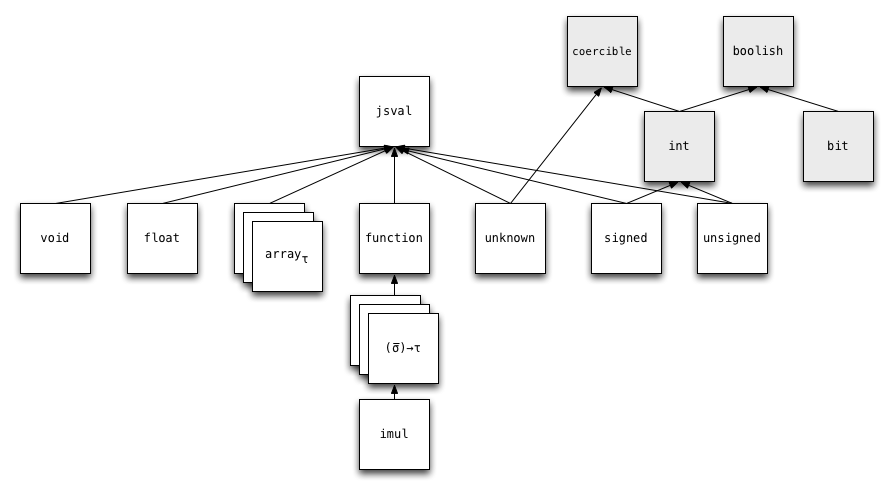
\includegraphics[scale=0.5]{subtypes}
\caption{The hierarchy of expression types.}
\label{fig:subtypes}
\end{figure}

\subsubsection*{The $\extern$ type}

This abstract type represents the root of all types that can escape
back into ordinary JavaScript. Any type that is a subtype of $\extern$
must carry enough information in its internal representation in an
optimizing virtual machine to faithfully convert back into a dynamic
JavaScript value.

\subsubsection*{The $\double$ type}

This is the type of double-precision floating-point values. An
optimizing engine can represent these as unboxed 64-bit floats. If
they escape into external JavaScript they must of course be wrapped
back up as JavaScript values according to the JavaScript engine's
value representation.

\subsubsection*{The $\signed$ and $\unsigned$ types}

These are the types of signed and unsigned 32-bit integers,
respectively. For an optimizing engine, their representation can be
the same: an unboxed 32-bit integer. If a value escapes into external
JavaScript, the sign is used to determine which JavaScript value it
represents. For example, the bit pattern $\mathjs{0xffffffff}$
represents either the JavaScript value $\mathjs{-1}$ or
$\mathjs{4294967295}$, depending on the signedness of the type.

\subsubsection*{The $\fixnum$ type}

This type represents integers in the range $[0, 2^{31})$, which are
both valid signed and unsigned integers. Literals in this range are
given the type $\fixnum$.

\subsubsection*{The $\int$ type}

This is the type of 32-bit integers whose sign is not known. Again,
optimizing engines can represent them as unboxed 32-bit integers. But
because the sign is not known, they cannot be allowed to escape to
external JavaScript, as it is impossible to determine exactly which
JavaScript value they represent. While this might not seem like a very
useful type, the JavaScript bitwise coercions can be used to force an
$\int$ value back to $\signed$ or $\unsigned$ without any loss of
data.

\subsubsection*{The $\intish$ type}

The JavaScript arithmetic operations can be performed on 32-bit
integer values, but their results may produce non-integer values. For
example, addition and subtraction can overflow to large numbers that
exceed the 32-bit integer range, and integer division can produce a
non-integer value. However, if the result is coerced back to an
integer, the resulting arithmetic operation behaves identically to the
typical corresponding machine operation (i.e., integer addition,
subtraction, or division). The $\intish$ type represents the result of
a JavaScript integer artihmetic operation that must be coerced back to
integer with an explicit coercion. Because this type can only be used
as an argument to a coercion (or silently ignored in an expression
statement), $\mathjs{asm.js}$ integer arithmetic can always be
implemented in an optimizing engine by the machine integer artithmetic
operations.

The one arithmetic operation that does not quite fit into this story
is multiplication. Multiplying two large integers can results in a
large enough double that some lower bits of precision are lost, so
that coercing the result back to integer does {\it not} behave
identically to the machine operation. The use of the proposed ES6
$\mathjs{Math.imul}$ function~\cite{imul} as an FFI function is
recommended as the proper means of implementing integer
multiplication.

\subsubsection*{The $\bit$ type}

The conditional operators produce boolean values in
JavaScript. Booleans are interconvertible to the JavaScript integer
values $\mathjs{0}$ and $\mathjs{1}$ via integer coercion and back via
boolean coercion. In order to allow optimizing engines to represent
these as untagged 32-bit integers, we disallow the $\bit$ type from
escaping to external JavaScript. The only contexts where they can be
used are in conditionals (such as the test expression of an
$\mathjs{if}$ statement), or in coercions to integer.

\subsubsection*{The $\boolish$ type}

Every type in JavaScript can be implicitly converted to a boolean for
the sake of evaluating a conditional expression or statement. This
coercion is allowed in $\mathjs{asm.js}$ for the $\bit$ type as well
as the integer types, but not for the $\double$ type. This ensures
that an optimizing JavaScript engine only ever performs a conditional
based on an unboxed 32-bit integer value, avoiding the need for a more
expensive conversion.

\subsubsection*{The $\unk$ type}

Calling an external JavaScript function through the FFI results in an
arbitrary JavaScript value. Because $\mathjs{asm.js}$ is designed to
avoid dealing with general values, the result must be coerced to one
of the other types before it can be used. The $\unk$ type represents
one of these result values before being coerced to an integer or
double.

\subsubsection*{The $\void$ type}

A function that returns $\mathjs{undefined}$ is considered to have the
$\void$ result type. The $\mathjs{undefined}$ value is not actually a
first-class value in $\mathjs{asm.js}$. It can only be ignored via an
expression statement. This avoids having to represent it at all as
data.

\subsection{Environment types}

Validation tracks the types not only of expressions and local
variables but also global variables, FFI imports, and functions. These
include typed arrays, the special $\mathjs{Math.imul}$ value, FFI
functions, and $\mathjs{asm.js}$ functions:
\[
\rho ::= \tau ~|~ \view{n}{\tau} ~|~ \imul ~|~ \function ~|~ \funty{\seq{\sigma}}{\tau}
\]

The type of a typed array tracks the number of bits per element and
the elements' value type ($\int$ or $\double$). The $\imul$ and
$\function$ types are straightforward. The type of a function define
within the $\mathjs{asm.js}$ module includes the types of its
parameters and its return type.

\subsection{Operator types}

\[
\omega ::= (\funty{\seq{\sigma}}{\tau}) \land \ldots \land (\funty{\seq{\sigma'}}{\tau'})
\]

\section{Type rules}

\[
\begin{array}{rcl}
\vartype(\todouble{x}), \vartype(r) & = & \double \\
\vartype(x\mathjs{|0}), \vartype(n) & = & \int \mbox{ $(-2^{31} \leq n < 2^{32})$} \\
\rettype(\todouble{e}), \rettype(r) & = & \double \\
\rettype(e\mathjs{|0}), \rettype(n) & = & \signed \mbox{ $(-2^{31} \leq n < 2^{31})$} \\
\rettype(\epsilon)                  & = & \void \\
\end{array}
\]

\[
\begin{array}{rcl}
M(\imul) & : & \imul \\
M(\mathtt{ceil}), M(\mathtt{sin}), M(\mathtt{cos}) & : & \funty{\double}{\double} \\
\end{array}
\]

\[
\begin{array}{rcl}
A(\mathtt{Uint8Array}), A(\mathtt{Int8Array})   & = & \view{8}{\intsm} \\
A(\mathtt{Uint16Array}), A(\mathtt{Int16Array}) & = & \view{16}{\intsm} \\
A(\mathtt{Uint32Array}), A(\mathtt{Int32Array}) & = & \view{32}{\intsm} \\
A(\mathtt{Float32Array})                        & = & \view{32}{\doublesm} \\
A(\mathtt{Float64Array})                        & = & \view{64}{\doublesm} \\
\end{array}
\]

\[
\begin{array}{rcc@{\ }l}
\mathjs{+}, \mathjs{-}
                 & : &       & \funty{\double, \double}{\double} \\
                 &   & \land & \funty{\int, \int}{\intish} \\
\mathjs{*}       & : &       & \funty{\double, \double}{\double} \\
\mathjs{/}, \mathjs{\%}
                 & : &       & \funty{\double, \double}{\double} \\
                 &   & \land & \funty{\signed, \signed}{\intish}  \\
                 &   & \land & \funty{\unsigned, \unsigned}{\intish} \\
\\
\mathjs{|}, \mathjs{\&}, \mathjs{\^{}}, \mathjs{<<}, \mathjs{>>}
                 & : &       & \funty{\intish, \intish}{\signed} \\
\mathjs{>>>}     & : &       & \funty{\intish, \intish}{\unsigned} \\
\\
\mathjs{<}, \mathjs{<=}, \mathjs{>}, \mathjs{>=}, \mathjs{==}, \mathjs{!=}
                 & : &       & \funty{\signed, \signed}{\bit} \\
                 &   & \land & \funty{\unsigned, \unsigned}{\bit} \\
                 &   & \land & \funty{\double, \double}{\bit} \\
\\
\mathjs{+}       & : &       & \funty{\intish}{\double} \\
\mathjs{\~{}}    & : &       & \funty{\intish}{\signed} \\
\mathjs{!}       & : &       & \funty{\boolish}{\bit} \\
\end{array}
\]

\[
\begin{array}{rcl}
\Delta & ::= & \{ \seq{x : \rho} \} \\
\Gamma & ::= & \{ \seq{x : \tau} \} \\
\end{array}
\]

\[
\begin{array}{l}
\funtype(\fun{f}{\seq{x}}{\seq{x\mathjs{ = }\mathit{ann}_x\mathjs{;}}\ \seq{\var{\seq{y\mathjs{ = }v}}}\ \mathit{ss}}) = \funty{\seq{\sigma}}{\tau} \\
\qquad \mbox{where } \forall i . \vartype(\mathit{ann}_{x_i}) = \sigma_i \\
\qquad \mbox{and } \forall \return{[\mathit{re}]} \in \mathit{ss} . \rettype([\mathit{re}]) = \tau
\end{array}
\]

\[
\begin{array}{rcl}
\breaks(\seq{s}) & = & \bigcup_i \breaks(s_i) \\
\breaks(\block{\mathit{ss}}) & = & \breaks(\mathit{ss}) \\
\breaks(\ifthen{e}{s}) & = & \breaks(s) \\
\breaks(\ifthenelse{e}{s_1}{s_2}) & = & \breaks(s_1) \cup \breaks(s_2) \\
\breaks(\while{e}{s}) & = & \breaks(s) - \{ \epsilon \} \\
\breaks(\dowhile{s}{e}) & = & \breaks(s) - \{ \epsilon \} \\
\breaks(\for{[e_1]}{[e_2]}{[e_3]}{s}) & = & \breaks(s) - \{ \epsilon \} \\
\breaks(\brk) & = & \{ \epsilon \} \\
\breaks(\brkl{\mathit{lab}}) & = & \{ \mathit{lab} \} \\
\breaks(\lab{\mathit{lab}}{s}) & = & \breaks(s) - \{ \mathit{lab} \} \\
\breaks(\switch{e}{\seq{\mathit{cd}}}) & = & \bigcup_i \breaks(\mathit{cd}_i) - \{ \epsilon \} \\
\breaks(s) \mbox{ (otherwise)} & = & \emptyset \\
\breaks(\mathjs{case }v\mathjs{:}\,\mathit{ss}) & = & \breaks(\mathit{ss}) \\
\breaks(\mathjs{default:}\,\mathit{ss}) & = & \breaks(\mathit{ss}) \\
\end{array}
\]

\[
\begin{array}{lr}
\mbox{Module checking} & \hfil \fbox{$\progjudge{\mathit{mod}}$}
\rulebreak
\multicolumn{2}{c}{
\begin{array}{c}
\inferrule* [lab=\rel{T-Program}]
  {\seq{x}, \seq{y}, \seq{f}, [g], [e], [b]\ \mbox{distinct} \\
   \Delta = \{ \seq{f : \funtype(\mathit{fn}_f)}, \seq{y : \vartype(v)} \} \\\\
   \forall i . \impjudge{[e]}{[b]}{\Delta}{\mathit{imp}_x} \\
   \forall i . \fnjudge{\Delta}{\mathit{fn}_f} \\
   \forall i . \expjudge{\Delta}{\mathit{exp}}}
  {\progjudge{\fun{[g]}{[e[, b]]}{\mathjs{"use asm";}\ \seq{\mathit{imp}_x}\ \seq{\mathit{fn}_f}\ \seq{\var{\seq{y \mathjs{ = } v}}}\ \mathit{exp}}}}
\end{array}
}
\\ \\
\mbox{Import checking} & \hfil \fbox{$\impjudge{[e]}{[b]}{\Delta}{\mathit{imp}}$}
\rulebreak
\multicolumn{2}{c}{
\begin{array}{c}
\inferrule* [lab=\rel{T-ImportStd}]
  {\Delta(x) = M(y)}
  {\impjudge{e}{[b]}{\Delta}{\var{x \mathjs{ = } e\mathjs{.}y}}}
\qquad
\inferrule* [lab=\rel{T-ImportFFI}]
  {y \not\in\dom(M), \dom(A) \\
   \Delta(x) = \function}
  {\impjudge{e}{[b]}{\Delta}{\var{x \mathjs{ = } e\mathjs{.}y}}}
\\ \\
\inferrule* [lab=\rel{T-View}]
  {\Delta(x) = \view{n}{A(y)}}
  {\impjudge{e}{b}{\Delta}{\var{x \mathjs{ = new } e\mathjs{.}y(b)}}}
\end{array}
}
\\ \\
\mbox{Function checking} & \hfil \fbox{$\fnjudge{\Delta}{\mathit{fn}}$}
\rulebreak
\multicolumn{2}{c}{
\begin{array}{c}
\inferrule* [lab=\rel{T-Function}]
  {\seq{x}, \seq{y}\ \mbox{distinct} \\
   \Delta(f) = \funty{\seq{\sigma}}{\tau} \\
   \seq{\sigma} = \seq{\vartype(\mathit{ann}_x)} \\\\
   \sjudge{\Delta}{\{ \seq{x : \sigma}, \seq{y : \vartype(v)} \}}{\mathit{ss}} \\
   \tau \not=\void \Rightarrow \returns(\mathit{ss})}
  {\fnjudge{\Delta}{\fun{f}{\seq{x}}{\seq{x\mathjs{ = }\mathit{ann}_x\mathjs{;}}\ \seq{\var{\seq{y\mathjs{ = }v}}}\ \mathit{ss}}}}
\end{array}
}
\\ \\
\mbox{Export checking} & \hfil \fbox{$\expjudge{\Delta}{\mathit{exp}}$}
\rulebreak
\multicolumn{2}{c}{
\begin{array}{c}
\inferrule* [lab=\rel{T-Singleton}]
  {\Delta(f) = \funty{\seq{\sigma}}{\tau} \\
   \tau <: \extern }
  {\expjudge{\Delta}{\return{f}}}
\qquad
\inferrule* [lab=\rel{T-Module}]
  {\forall f . \Delta(f) = \funty{\seq{\sigma}}{\tau} \land
   \tau <: \extern}
  {\expjudge{\Delta}{\return{\mathjs{\char123{} } \seq{x \mathjs{:} f} \mathjs{ \char125{}}}}}
\end{array}
}
\end{array}
\]

\newsavebox{\switchcontrol}
\begin{lrbox}{\switchcontrol}
\begin{minipage}[t]{2.87in}
\vspace{-.25in}
\[
\varepsilon = \left\{ \begin{array}{ll}
                      \mustret & \mbox{if}\ \varepsilon_n = \mustret \land \forall i . \varepsilon_i \cup \emptyset = \emptyset \\
                      \bigcup \varepsilon_i - \{ \epsilon \} & \mbox{otherwise}
                      \end{array} \right.
\]
\end{minipage}
\end{lrbox}

\[
\begin{array}{l}
\returns(\seq{s}) \\
\qquad \mbox{if } \returns(s_m) \land \forall i < m . \breaks(s_m) = \emptyset \mbox{ for some } m \\
\returns(\block{\mathit{ss}}) \\
\qquad \mbox{if } \returns(ss) \\
\returns(\ifthenelse{e}{s_1}{s_2}) \\
\qquad \mbox{if } \returns(s_1) \land \returns(s_2) \\
\returns(\dowhile{s}{e}) \\
\qquad \mbox{if } \returns(s) \\
\returns(\switch{e}{\seq{\mathit{cd}}}) \\
\qquad \mbox{if } \returns(cd_n) \land \forall i . \breaks(cd_i) = \emptyset \\
\returns(\mathjs{case }v\mathjs{:}\,\mathit{ss}) \\
\qquad \mbox{if } \returns(\mathit{ss}) \\
\returns(\mathjs{default:}\,\mathit{ss}) \\
\qquad \mbox{if } \returns(\mathit{ss})
\end{array}
\]

\[
\begin{array}{lr}
\mbox{Statement list checking} & \hfil \fbox{$\sjudge{\Delta}{\Gamma}{\mathit{ss}}$}
\rulebreak
\multicolumn{2}{c}{
\begin{array}{c}
\inferrule* [lab=\rel{T-Statements}]
  {\forall i . \sjudge{\Delta}{\Gamma}{s_i}}
  {\sjudge{\Delta}{\Gamma}{\seq{s}}}
\end{array}
}
\\ \\
\mbox{Statement checking} & \hfil \fbox{$\sjudge{\Delta}{\Gamma}{s}$}
\rulebreak
\multicolumn{2}{c}{
\begin{array}{c}
\inferrule* [lab=\rel{T-Block}]
  {\sjudge{\Delta}{\Gamma}{\mathit{ss}}}
  {\sjudge{\Delta}{\Gamma}{\block{\mathit{ss}}}}
\qquad
\inferrule* [lab=\rel{T-ExprStmt}]
  {\exprjudge{\Delta}{\Gamma}{e}{\sigma}}
  {\sjudge{\Delta}{\Gamma}{e\mathjs{;}}}
\qquad
\inferrule* [lab=\rel{T-EmptyStatement}]
  { }
  {\sjudge{\Delta}{\Gamma}{\mathjs{;}}}
\\ \\
\inferrule* [lab=\rel{T-If}]
  {\exprjudge{\Delta}{\Gamma}{e}{\boolish} \\\\
   \sjudge{\Delta}{\Gamma}{s}}
  {\sjudge{\Delta}{\Gamma}{\ifthen{e}{s}}}
\qquad
\inferrule* [lab=\rel{T-IfElse}]
  {\exprjudge{\Delta}{\Gamma}{e}{\boolish} \\\\
   \sjudge{\Delta}{\Gamma}{s_1} \\
   \sjudge{\Delta}{\Gamma}{s_2}}
  {\sjudge{\Delta}{\Gamma}{\ifthenelse{e}{s_1}{s_2}}}
\\ \\
\inferrule* [lab=\rel{T-ReturnExpr}]
  {\exprjudge{\Delta}{\Gamma}{\mathit{re}}{\tau} \\
   \rettype(\mathit{re}) = \tau}
  {\sjudge{\Delta}{\Gamma}{\return{\mathit{re}}}}
\qquad
\inferrule* [lab=\rel{T-ReturnVoid}]
  { }
  {\sjudge{\Delta}{\Gamma}{\mathtt{return;}}}
\\ \\
\inferrule* [lab=\rel{T-While}]
  {\exprjudge{\Delta}{\Gamma}{e}{\boolish} \\\\
   \sjudge{\Delta}{\Gamma}{s}}
  {\sjudge{\Delta}{\Gamma}{\while{e}{s}}}
\qquad
\inferrule* [lab=\rel{T-DoWhile}]
  {\sjudge{\Delta}{\Gamma}{s} \\\\
   \exprjudge{\Delta}{\Gamma}{e}{\boolish}}
  {\sjudge{\Delta}{\Gamma}{\dowhile{s}{e}}}
\\ \\
\inferrule* [lab=\rel{T-For}]
  {[\exprjudge{\Delta}{\Gamma}{e_1}{\sigma_1}] \\
   [\exprjudge{\Delta}{\Gamma}{e_2}{\boolish}] \\
   [\exprjudge{\Delta}{\Gamma}{e_3}{\sigma_3}] \\\\
   \sjudge{\Delta}{\Gamma}{s}}
  {\sjudge{\Delta}{\Gamma}{\for{[e_1]}{[e_2]}{[e_3]}{s}}}
\\ \\
\inferrule* [lab=\rel{T-Break}]
  { }
  {\sjudge{\Delta}{\Gamma}{\brkl{[\mathit{lab}]}}}
\qquad
\inferrule* [lab=\rel{T-Continue}]
  { }
  {\sjudge{\Delta}{\Gamma}{\contl{[\mathit{lab}]}}}
\\ \\
\inferrule* [lab=\rel{T-Label}]
  {\sjudge{\Delta}{\Gamma}{s}}
  {\sjudge{\Delta}{\Gamma}{\lab{\mathit{lab}}{s}}}
\qquad
\inferrule* [lab=\rel{T-Switch}]
  {\exprjudge{\Delta}{\Gamma}{e}{\sigma} \\
   \sigma <: \extern \\
   \forall i . \exprjudge{\Delta}{\Gamma}{v_i}{\sigma} \\\\
   \forall i . \sjudge{\Delta}{\Gamma}{\mathit{ss}_i} \\
   [\sjudge{\Delta}{\Gamma}{\mathit{ss}}]}
  {\sjudge{\Delta}{\Gamma}{\switch{e}{\seq{\mathjs{case }v_i\mathjs{:}\,\mathit{ss}_i}\ [\mathjs{default:}\,\mathit{ss}]}}}
\end{array}
}
\end{array}
\]

\[
\begin{array}{lr}
\mbox{Case checking} & \hfil \fbox{$\sjudge{\Delta}{\Gamma}{\mathit{cd}}$}
\rulebreak
\multicolumn{2}{c}{
\begin{array}{c}
\inferrule* [lab=\rel{T-Case}]
  {\sjudge{\Delta}{\Gamma}{\mathit{ss}}}
  {\sjudge{\Delta}{\Gamma}{\mathjs{case }v\mathjs{:}\,\mathit{ss}}}
\qquad
\inferrule* [lab=\rel{T-Default}]
  {\sjudge{\Delta}{\Gamma}{\mathit{ss}}}
  {\sjudge{\Delta}{\Gamma}{\mathjs{default:}\,\mathit{ss}}}
\end{array}
}
\end{array}
\]

\[
(\Delta\cdot\Gamma)(x) = \left\{\begin{array}{ll}
                                \Gamma(x) & \mbox{if}\ x \in\dom(\Gamma) \\
                                \Delta(x) & \mbox{otherwise}
                                \end{array} \right.
\]

\[
\begin{array}{lr}
\mbox{Expression checking} & \hfil \fbox{$\exprjudge{\Delta}{\Gamma}{e}{\tau}$}
\rulebreak
\multicolumn{2}{c}{
\begin{array}{c}
\inferrule* [lab=\rel{T-Signed}]
  {-2^{31} \leq n < 0}
  {\exprjudge{\Delta}{\Gamma}{n}{\signed}}
\qquad
\inferrule* [lab=\rel{T-Fixnum}]
  {0 \leq n < 2^{31}}
  {\exprjudge{\Delta}{\Gamma}{n}{\fixnum}}
\qquad
\inferrule* [lab=\rel{T-Unsigned}]
  {2^{31} \leq n < 2^{32}}
  {\exprjudge{\Delta}{\Gamma}{n}{\unsigned}}
\\ \\
\inferrule* [lab=\rel{T-Double}]
  { }
  {\exprjudge{\Delta}{\Gamma}{r}{\double}}
\qquad
\inferrule* [lab=\rel{T-VarRef}]
  {(\Delta\cdot\Gamma)(x) = \tau}
  {\exprjudge{\Delta}{\Gamma}{x}{\tau}}
\qquad
\inferrule* [lab=\rel{T-Assign}]
  {\exprjudge{\Delta}{\Gamma}{e}{\tau} \\
   \tau <: (\Delta\cdot\Gamma)(x)}
  {\exprjudge{\Delta}{\Gamma}{x\mathjs{ = }e}{\tau}}
\\ \\
\inferrule* [lab=\rel{T-Load}]
  {m = 2^k - 1 \\
   (\Delta\cdot\Gamma)(x) = \view{n}{\tau} \\\\
   \exprjudge{\Delta}{\Gamma}{e}{\intish}}
  {\exprjudge{\Delta}{\Gamma}{\getprop{x}{\paren{e\mathjs{ \& } m}\mathjs{ >> }n/8}}{\tau}}
\qquad
\inferrule* [lab=\rel{T-Store}]
  {m = 2^k - 1 \\
   (\Delta\cdot\Gamma)(x) = \view{n}{\tau} \\\\
   \exprjudge{\Delta}{\Gamma}{e_1}{\intish} \\
   \exprjudge{\Delta}{\Gamma}{e_2}{\tau}}
  {\exprjudge{\Delta}{\Gamma}{\getprop{x}{\paren{e_1\mathjs{ \& } m}\mathjs{ >> }n/8}\mathjs{ = }e_2}{\tau}}
\\ \\
\inferrule* [lab=\rel{T-IMul}]
  {(\Delta\cdot\Gamma)(f) = \imul \\\\
   \forall i . \exprjudge{\Delta}{\Gamma}{e_i}{\intish}}
  {\exprjudge{\Delta}{\Gamma}{\funcall{f}{e_1, e_2}}{\signed}}
\qquad
\inferrule* [lab=\rel{T-FunCall}]
  {(\Delta\cdot\Gamma)(f) = \funty{\seq{\sigma}}{\tau} \\\\
   \forall i . \exprjudge{\Delta}{\Gamma}{e_i}{\sigma_i}}
  {\exprjudge{\Delta}{\Gamma}{\funcall{f}{\seq{e}}}{\tau}}
\qquad
\inferrule* [lab=\rel{T-FFI}]
  {(\Delta\cdot\Gamma)(f) = \function \\\\
   \forall i . \exprjudge{\Delta}{\Gamma}{e_i}{\extern}}
  {\exprjudge{\Delta}{\Gamma}{\funcall{f}{\seq{e}}}{\unk}}
\\ \\
\inferrule* [lab=\rel{T-Conditional}]
  {\exprjudge{\Delta}{\Gamma}{e_1}{\boolish} \\\\
   \exprjudge{\Delta}{\Gamma}{e_2}{\tau} \\
   \exprjudge{\Delta}{\Gamma}{e_3}{\tau}}
  {\exprjudge{\Delta}{\Gamma}{\ternary{e_1}{e_2}{e_3}}{\tau}}
\qquad
\inferrule* [lab=\rel{T-Paren}]
  {\forall i \leq n . \exprjudge{\Delta}{\Gamma}{e_i}{\tau_i}}
  {\exprjudge{\Delta}{\Gamma}{\paren{\seq{e}}}{\tau_n}}
\\ \\
\inferrule* [lab=\rel{T-Unop}]
  {\mathit{unop} : \_ \land \funty{\sigma}{\tau} \land \_ \\
   \exprjudge{\Delta}{\Gamma}{e}{\sigma}}
  {\exprjudge{\Delta}{\Gamma}{\mathit{unop}\ e}{\tau}}
\qquad
\inferrule* [lab=\rel{T-Binop}]
  {\mathit{binop} : \_ \land \funty{\sigma_1, \sigma_2}{\tau} \land \_ \\\\
   \exprjudge{\Delta}{\Gamma}{e_1}{\sigma_1} \\
   \exprjudge{\Delta}{\Gamma}{e_2}{\sigma_2}}
  {\exprjudge{\Delta}{\Gamma}{e_1\ \mathit{binop}\ e_2}{\tau}}
\\ \\
\inferrule* [lab=\rel{T-Sub}]
  {\exprjudge{\Delta}{\Gamma}{e}{\sigma} \\
   \sigma <: \tau}
  {\exprjudge{\Delta}{\Gamma}{e}{\tau}}
\qquad
\inferrule* [lab=\rel{T-Cast}]
  {\exprjudge{\Delta}{\Gamma}{e}{\double}}
  {\exprjudge{\Delta}{\Gamma}{\mathjs{\~{}\~{}}e}{\signed}}
\end{array}
}
\end{array}
\]

\end{document}
